% Section III -- System Description and Data
% Draft 1 (22 Nov 2026). Numbers from inputs/inputs_summary.md, docs/data_inventory.md and
% docs/assumption_register.md in the GitHub repository; figures from tools/make_paper_figs.py.
\section{System Description and Data}
\label{sec:system}

No metered load, fuel or outage records were available for the club, so every input in this
study is taken from public data or derived from it. The load is therefore reconstructed bottom-up and carried as low, base, and high scenarios rather
than as a single estimate. Each input is labelled as verified (stated by a
source), derived (computed from cited inputs), or assumed; the full register, with a source for
every value, is published with the model code.\footnote{\url{https://github.com/Joe-Sfeir/MicrogridProject}} The study is therefore a scenario-based feasibility assessment, and its conclusions are
tested against the spread of these scenarios in Section~V.

\subsection{Site}
Faqra Club lies in Kfardebian, Keserwan (33.985\,$^\circ$N, 35.811\,$^\circ$E), between 1,735 and
1,975~m above sea level (Fig.~\ref{fig:site}). Its four lifts are a chairlift (T1, 880~m long with a
240~m rise) and three surface lifts (T2--T4)~\cite{skiresort}. The resort also comprises a 25-key
hotel, three restaurants, a swimming pool, sports grounds, a water supply and wastewater plant,
about 20~km of lit private roads, and 350--400 privately owned chalets~\cite{faqraabout}. The ski
season runs from about mid-December to March, with 80 operating days in the base case.

\begin{figure}[!t]
\centering
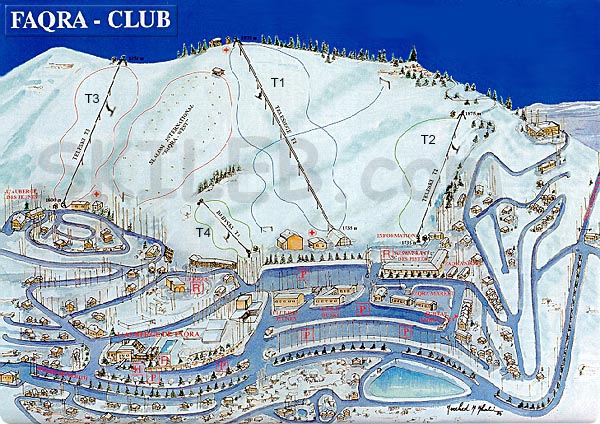
\includegraphics[width=\columnwidth]{figs/faqra_trailmap.jpg}
\caption{Faqra Club site layout showing the ski lifts (T1--T4), chalets, and parking areas.
[Source: Faqra Club, reproduced with permission.]}
\label{fig:site}
\end{figure}

\subsection{Load Reconstruction}
The hourly demand is built from twelve load blocks $i$:
\begin{equation}
P_L(t) = \sum_{i} N_i \, P_{\mathrm{rated},i} \, f_i(t),
\label{eq:load}
\end{equation}
where $N_i$ is the number of units of block $i$, $P_{\mathrm{rated},i}$ their rated power, and
$f_i(t)\in[0,1]$ an hourly utilization factor that depends on the hour, the day type (weekday or
weekend/holiday), and the season. Table~\ref{tab:load} lists the blocks and their main sources.

\emph{Ski lifts.} The lift power is computed from the work of lifting skiers ($mgH$, with ski friction
on the surface lifts) and from a no-load share for the rope and drive, scaled by measured chairlift
data from Madonna di Campiglio~\cite{viesi2023} and the no-load share reported in~\cite{blasuttigh2023}.
Lebanon records about 300,000 skier visits per year;
allocating the visits outside Mzaar by lift gives about 10,700 skier-days for Faqra. Because traffic
is light, 86--94\% of the lift energy is no-load running, so the number of lifts in service matters
more than the number of skiers.

\emph{Hotel, restaurants and chalets.} Hotel and restaurant demand follows published energy-use
intensities and schedules, with monthly occupancy taken from
Lebanese tourism data. Chalet demand uses Lebanese household consumption per occupied
day and an assumed 100 occupied days per year, typical of second homes in
mountain resorts. The chalets are the largest block, so the study
also reports a club-only boundary.

\emph{Auxiliary loads.} Road lighting assumes LED poles operated from dusk to dawn with dimming after
midnight; water pumping follows per-capita demand and the energy intensity of lifting
groundwater, and the wastewater plant uses the treatment intensity from the same
review. Sports lighting, the pool, an electric-vehicle charger, security and offices make up the
remainder.

\begin{table}[!t]
\centering
\caption{Annual Energy of the Reconstructed Load (MWh/yr)}
\label{tab:load}
\footnotesize
\setlength{\tabcolsep}{3pt}
\begin{tabular}{@{}l r r r c@{}}
\toprule
Block & Low & Base & High & Critical share \\
\midrule
Chalets (350--400)            & 443 & 932   & 2,076 & 0\%   \\
Ski lifts (T1--T4)            & 21  & 57    & 120   & 0\%   \\
Hotel (25 keys)               & 49  & 119   & 233   & 30\%  \\
Restaurants (3)               & 31  & 111   & 369   & 30\%  \\
Road lighting (20 km)         & 53  & 93    & 232   & 30\%  \\
Water pumping                 & 7   & 39    & 153   & 100\% \\
Wastewater plant              & 4   & 14    & 51    & 100\% \\
Sports, pool, EV, offices     & 18  & 67    & 152   & 0--30\% \\
Security                      & 13  & 26    & 50    & 100\% \\
\midrule
Total                         & 639 & 1,457 & 3,434 & \\
Peak (kW)                     & 220 & 519   & 1,066 & \\
Critical energy               & 67  & 184   & 518   & \\
\bottomrule
\end{tabular}
\end{table}

\emph{Critical load.} Loads are grouped by the priority classes of emergency and standby
systems. Water supply, wastewater treatment, and security are fully critical. A
share of 30\% of the hotel, restaurant, road-lighting and office load is critical, which matches the
critical fraction used in resilience studies. The lifts, chalets, pool, sports
lighting and vehicle charging can be shed. The critical load must always be served, while the
remaining load may only be shed within the reliability limit of Section~IV.

Figure~\ref{fig:loadmonthly} shows the monthly energy of the base case. Demand has two seasons: a
winter peak driven by skiing and chalet occupancy, and a smaller summer peak from chalet occupancy
and outdoor activity. Spring and autumn demand is less than half of January's. The coincident peak of
519~kW occurs at 13:00 on the busiest ski Saturday, when lifts, restaurants and occupied chalets
overlap (Fig.~\ref{fig:loaddays}).

\begin{figure}[!t]
\centering
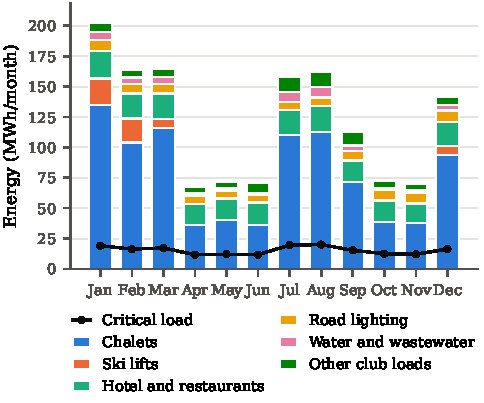
\includegraphics[width=\columnwidth]{figs/load_monthly.pdf}
\caption{Monthly energy of the base-case load by block, and its critical part.}
\label{fig:loadmonthly}
\end{figure}

\begin{figure}[!t]
\centering
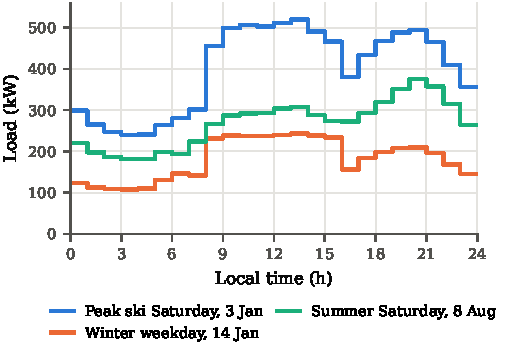
\includegraphics[width=\columnwidth]{figs/load_days.pdf}
\caption{Hourly base-case load on three characteristic days.}
\label{fig:loaddays}
\end{figure}

\subsection{Solar Resource and Snow}
Hourly PV output per installed kWp is taken from PVGIS for 2014--2023, with the SARAH-3 satellite
irradiance, the local horizon, crystalline-silicon modules, and 14\% system losses.\footnote{\url{https://joint-research-centre.ec.europa.eu/pvgis}}
Satellite and reanalysis sources agree within about 5\% from May to September, but differ by 30--40\%
from December to March: PVGIS notes that snow-covered ground can be mistaken for cloud, which biases
SARAH low in winter, while ERA5 tends to read high in mountain terrain.
A third source, the Solargis long-term means of the Global Solar Atlas,\footnote{\url{https://globalsolaratlas.info}} lies between
the two. With no ground station available, the base case applies the monthly bias correction that is
the simplest form of site adaptation: each hour of the SARAH-3 series is scaled by the
ratio of the Solargis and SARAH-3 monthly irradiance,
\begin{equation}
a(t) = k_{m(t)} \, a_{\mathrm{SARAH}}(t), \qquad
k_m = \frac{\overline{G}_{\mathrm{Solargis},m}}{\overline{G}_{\mathrm{SARAH},m}},
\label{eq:scale}
\end{equation}
where $a(t)$ is the PV output per kWp and $k_m$ ranges from 0.99 in September to 1.24 in January. The
unscaled SARAH-3 series and the PVGIS-ERA5 series serve as the low and high irradiance cases
(Fig.~\ref{fig:pv}). The representative year is 2015, the year closest to the 2014--2023 mean in both
annual and December--March yield; the other nine years are used in the robustness
check of Section~V.

Snow on the modules is modelled with the snow-coverage method of Marion \textit{et al.}~\cite{marion2013}
in its hourly form. The array is fully covered in any hour with at least 1~cm of
snowfall. Snow slides off at $0.197\sin\beta$ of the array height per hour, where $\beta$ is the tilt,
whenever the air temperature exceeds $G_{\mathrm{POA}}/m$ with $m=-80$~W\,m$^{-2}$\,$^\circ$C$^{-1}$,
and the output is reduced by the covered fraction. Hourly temperature comes from
ERA5-Land and precipitation from ERA5; precipitation is
counted as snow below 1.0\,$^\circ$C, with a snow-to-liquid ratio of 10:1. The
resulting December--March loss is 3.5--4.6\% depending on tilt, and the base-case yield at 30$^\circ$
is 1,527~kWh/kWp per year. Snow losses of 0\% and 15\% are tested as bounds.

\begin{figure}[!t]
\centering
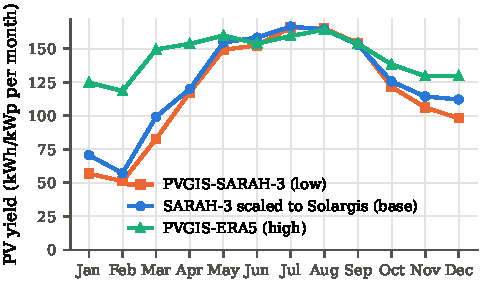
\includegraphics[width=\columnwidth]{figs/pv_monthly.pdf}
\caption{Monthly PV yield at 40$^\circ$ tilt, with snow losses, in the representative year 2015 for the
three irradiance cases.}
\label{fig:pv}
\end{figure}

\subsection{Grid Availability}
\'{E}lectricit\'{e} du Liban (EDL) publishes hourly energization records for each 20~kV feeder. The
record of the Faqra feeder of the Faitroun substation covers December 2024 to October
2026;\footnote{\url{https://edl.gov.lb/feeding.php}} the club is assumed to be supplied from this feeder. Over the 699 days the
feeder was energized 9.7~h/day on average, 10\% of days had no supply at all, and seven outages lasted
72~h or longer. Supply comes in irregular blocks rather than on a fixed schedule
(Fig.~\ref{fig:grid}). The model uses the most recent full year, November 2025 to October 2026
(8.1~h/day), as the binary availability $u_g(t)$. Fixed daily blocks of 4, 8 and 12~h, a case with no
grid, and an added 72~h outage in the peak ski week are tested as alternatives. Energy from EDL is
billed at a flat \$0.27/kWh plus a capacity charge, with no time-of-use rate.

\begin{figure}[!t]
\centering
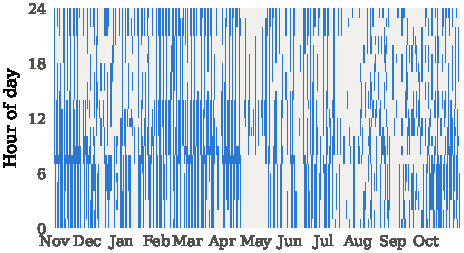
\includegraphics[width=\columnwidth]{figs/grid_heatmap.pdf}
\caption{Hours in which the Faqra feeder was energized (blue), November 2025 to October 2026
(mean 8.1~h/day).}
\label{fig:grid}
\end{figure}

\subsection{Diesel Generators}
The club's existing diesel generators supply the load whenever the grid is off. They are retained as
backup and treated as a sunk cost; a case in which they must be replaced at \$750/kW is tested
separately. Fuel use follows the standard linear fuel curve
\begin{equation}
F(t) = \alpha \, P_{\mathrm{com}}(t) + \beta \, P_{dg}(t),
\label{eq:fuel}
\end{equation}
where $P_{\mathrm{com}}$ is the committed capacity and $P_{dg}$ the output, with $\alpha=0.017$~L/h per kW
and $\beta=0.242$~L/kWh fitted to manufacturer data for six sets of 250--770~kVA. The base diesel price is
\$1.41/L, the 2026 Lebanese retail level~\cite{lorient2026}.

\subsection{Techno-Economic Parameters}
Table~\ref{tab:param} lists the component parameters. Costs are in 2025--2026 US dollars, and
annualization uses a real discount rate of 7.1\%, within the range reported for renewable projects
in Lebanon. The battery price of \$192/kWh is the 2025 installed cost of
lithium iron phosphate systems; the value of \$350/kWh used in the course
example is kept as a sensitivity. The battery power rating is limited to 0.5C.

\begin{table}[!t]
\centering
\caption{Techno-Economic Parameters (Base, with Low--High Range)}
\label{tab:param}
\footnotesize
\setlength{\tabcolsep}{4pt}
\begin{tabular}{@{}l l@{}}
\toprule
Parameter & Base (range) \\
\midrule
PV capital cost~\cite{lcec2025}        & \$750/kWp (600--1,003) \\
PV O\&M, life, degradation & \$18/kW-yr; 30~yr; 0.7\%/yr \\
BESS capital cost & \$192/kWh (125--334) \\
BESS O\&M, calendar life   & 2.5\% of capex/yr; 15~yr \\
Round-trip efficiency, SOC window      & 90\% (85--93); 10--100\% \\
Degradation cost~\cite{seger2023}      & \$0.020/kWh discharged \\
Diesel price~\cite{lorient2026}        & \$1.41/L (0.80--1.52) \\
Diesel O\&M; minimum load              & \$0.013/kWh; 30\% \\
EDL energy tariff & \$0.27/kWh \\
Real discount rate    & 7.1\% (5.8--12.4) \\
CO$_2$, diesel / grid                  & 2.68~kg/L; 0.70~kg/kWh \\
\bottomrule
\multicolumn{2}{@{}p{0.95\columnwidth}@{}}{\scriptsize Sources and derivations for every value are listed in the assumption register published with the model code.}
\end{tabular}
\end{table}
